
\documentclass{article}
\usepackage[utf8]{inputenc}

\title{RM Econometrics and Statistics}
\author{Clara Brünn, Christopher Thiemann and David Poth }
\date{October 2018}

\usepackage{natbib}
\usepackage{listings}
\usepackage{graphicx}
\usepackage{amssymb,amsfonts,amsthm,mathtools}
\usepackage{tikz}
\usepackage{url} % needed for waf
\usepackage{todonotes}
\usepackage{bbm}
\usepackage{booktabs}
%\usepackage[colorlinks,
%pdfpagelabels,
%pdfstartview = FitH,
%bookmarksopen = true,
%bookmarksnumbered = true,
%linkcolor = black,
%plainpages = false,
%hypertexnames = false,
%citecolor = black] {hyperref}    %This package enables links to sections from table of contents etc.
\theoremstyle{definition}
\newtheorem{theorem}{Theorem}
\newtheorem{definition}[theorem]{Definition}
\newtheorem{lemma}[theorem]{Lemma}
\DeclareMathOperator*{\argmin}{arg\,min}
\DeclareMathOperator*{\sgn}{sgn}
\bibliographystyle{ecta}
\begin{document}


\begin{titlepage} % Suppresses displaying the page number on the title page and the subsequent page counts as page 1
	\newcommand{\HRule}{\rule{\linewidth}{0.5mm}} % Defines a new command for horizontal lines, change thickness here
	
	\center % Centre everything on the page
	
	%------------------------------------------------
	%	Headings
	%------------------------------------------------
	
	\textsc{\LARGE University of Bonn}\\[1.5cm] % Main heading such as the name of your university/college
	
	\textsc{\Large Research Module Econometrics and Statistics}\\[0.5cm] % Major heading such as course name
	
	\textsc{\large Term paper}\\[0.5cm] % Minor heading such as course title
	
	%------------------------------------------------
	%	Title
	%------------------------------------------------
	
	\HRule\\[0.4cm]
	
	{\huge\bfseries Fused Lasso}\\[0.4cm] % Title of your document
	
	\HRule\\[1.5cm]
	
	%------------------------------------------------
	%	Author(s)
	%------------------------------------------------
	
	\begin{minipage}{0.4\textwidth}
		\begin{flushleft}
			\large
			\textit{Author's}\\
			Clara  	\textsc{Brünn} \newline
			David   \textsc{Poth} \newline
			Christopher	\textsc{Thiemann genannt Trappmann}% Your name
		\end{flushleft}
	\end{minipage}
	~
	\begin{minipage}{0.4\textwidth}
		\begin{flushright}
			\large
			\textit{Supervisor}\\
			Prof. Dr. Dominik \textsc{Liebl} % Supervisor's name
		\end{flushright}
	\end{minipage}
	
	% If you don't want a supervisor, uncomment the two lines below and comment the code above
	%{\large\textit{Author}}\\
	%John \textsc{Smith} % Your name
	
	%------------------------------------------------
	%	Date
	%------------------------------------------------
	
	\vfill\vfill\vfill % Position the date 3/4 down the remaining page
	
	{\large\today} % Date, change the \today to a set date if you want to be precise
	
	%------------------------------------------------
	%	Logo
	%------------------------------------------------
	
	%\vfill\vfill
	%\includegraphics[width=0.2\textwidth]{placeholder.jpg}\\[1cm] % Include a department/university logo - this will require the graphicx package
	 
	%----------------------------------------------------------------------------------------
	
	\vfill % Push the date up 1/4 of the remaining page
	
\end{titlepage} \newpage

\pagenumbering{Roman}

\tableofcontents \newpage

\addcontentsline{toc}{section}{List of Figures}

\listoffigures \newpage

\addcontentsline{toc}{section}{List of Tables}

\listoftables \newpage

\pagenumbering{arabic}


\section{Introduction}
TEST1234Methods for dealing with high-dimensional data are becoming more and more important in nearly all sciences among these empirical economics. This is due to the fact that data nowadays is often high-dimensional, i.e. it has a (much) larger number of variables than observations.

When analyzing high-dimensional data traditional methods as ordinary least squares turn out not to be appropriate. With traditional methods one is likely to encounter infeasible computation times, non-unique solutions and overfitting. Without constraints the OLS estimator would for example fit the data perfectly for $p=n$, resulting in probably weak out-of-sample forecasts. The reason is that the fit “captures not only the signal about how predictor variables may be used to forecast the outcome, but also fits the noise that is present in the given sample”, i.e. the model is overfit.
Therefore in order to analyze high-dimensional data “regularization” becomes necessary. This means one needs a dimension reduction, i.e. the estimates need to be constrained in order to avoid overfitting.  \citep{belloni2014}.

This paper examines one of the famous methods for dealing with this kind of set-up, the Lasso estimator and a modification of it, the fused lasso estimator.

NUR ZUM  VERANSCHAULICHUNG \includegraphics[width=\textwidth]{../../out/figures/simulation_dual.png}

\includegraphics[width=\textwidth]{../../out/figures/simulation_primal.png}



% Historical context
The Lasso was introduced by \citet{lasso}. Thereafter a lot of extensions were and still are being proposed. The most prominent are the elastic net by \citet{zou2005regularization}, the fused lasso by \citet{fused}, the adaptive lasso by \citet{zou2006adaptive} and  the group lasso by \citet{meier2008group}. Recent literature combines these extensions for example  \citet{bleakley2011group} present the grouped fused lasso.

The aim of this paper is to give a brief overview of the Lasso and Fused Lasso estimator and to analyze their properties in a simulation study and in a real data application. 

%Structure
The paper is organized as follows. We start by introducing the lasso. We define the optimization problem and give some properties thereof. After that we take a closer look at the estimator itself and show some basic properties and give intuitive explanations for the more advanced properties. We will also state some asymptotic results. The end of this chapter will give an idea on how to compute the estimator. The next chapter will then focus on the fused lasso which will be handled in a similar way as the lasso. We will compare both estimators in simulation studies and apply them to real data.


\todo{Write the introduction with a more detailed description of the historical context (elements of statistical learning) and a more detailed description of the steps in the paper}


\newpage

\section{Lasso}
\subsection{Definition and set-up}
We consider the linear regression model

\begin{equation}
	Y=X\beta+\varepsilon\quad,
\end{equation}
%
where $Y=(y_{1},...,y_{N})^T$ is the vector of responses, $X$ is the fixed $N \times p$ design matrix, $\beta=(\beta_1,...,\beta_p)^T$ a vector of parameters of interest and $\varepsilon=(\varepsilon_1,...,\varepsilon_N)^T$ a vector of i.i.d. error terms $\varepsilon_i \sim N(0,\sigma^2)$.\\
In contrast to the standard OLS setting, consider a high dimensional setting. This means that $p$ is much larger then $N$, which is denoted as $p>>N$. In that case $X$ does not have full rank and therefore the least squares estimate does not yield a unique solution. However there are cases where this obstacle can be overcome. In some cases (e.g. model selection), only a few of the $p$ included features are assumed relevant, such that $p_{relevant}\leq N$. This is called the 'sparsity' assumption.\\
The Lasso estimator exploits the 'sparsity' assumption by adding a penalty term on the non-zero regression parameters to the least squares estimator. Let $\lambda>0$ be the penalty constant, the the lasso estimator is defined as follows.

\begin{align}
\hat{\beta}_{\lambda}^{Lasso}&\in\argmin_{\beta \in\rm \mathbb{R}^p} \left \{ \frac{1}{2n}  \sum_{i=1}^{N}(y_{i}-x_{i}'\beta)^2+\lambda \sum_{j=1}^p|\beta_j| \right\}\\
\shortintertext{In matrix notation we can write this more compactly as}
\hat{\beta}_{\lambda}^{Lasso}&\in\argmin_{\beta \in\rm \mathbb{R}^p}  \left\{\frac{1}{2n} \| Y-X\beta\|_2^2+\lambda \| \beta\|_1 \right\}, \label{LassoLambda}
\end{align} 

\noindent where $ \| \cdot \|_2^2 $ is the squared Euclidean norm. This is equivalent to a constrained minimization problem of the form 

\begin{equation}
\hat{\beta}_{Primal}(R)=\argmin_{\beta:||\beta||_1\leq R} \frac{1}{n}||Y-X\beta||_2^2 \label{Primal}
\end{equation} 

\noindent where $R = \frac{||Y||^2}{\lambda}$, thus $R$ is dependent on the data and on $\lambda$.\footnote{See the appendix for details.}
% This result comes from convex optimization theory and we can apply it because $\frac{1}{n}||Y-X\beta||_2^2$ is convex in $\beta$ and $||\beta||_1\leq R$ a convex set.

Lasso regression puts constraints on the size of the coefficients associated to each variable. The solution should not depend on the measurement scale and this is why we normalize regressors and observations as follows. We replace $x_{i,j}$ by $x_{i,j}/ (\frac{1}{n} \sum_{i=1}^{n} x_{i,j}^2)^\frac{1}{2}$, thus the empirical standard deviation of each regressor is one. In order to have the same model equation as before replace $\beta_j$ with $(\frac{1}{n}\sum_{i=1}^{n} x_{i,j}^2)^\frac{1}{2} \beta_j$. Also we center the observations, i.e. they have mean zero, so that the intercept in the regression can be omitted. This is important since we do not want to shrink and punish the intercept as this does not prevent overfitting.


\subsection{Properties}
%Lasso sets to zero

\subsubsection{The penalty constant}

The penalty constant is a user-specified parameter, which is often chosen by a model selection procedure such as cross-validation \citep{sparsity}.
As the penalty constant $\lambda$ enters positively we can think about it as a cost for having $\hat{\beta_j}$'s unequal to zero. As $\lambda$ goes to infinity the resulting estimator will be a zero vector i.e $\hat{\beta}_{\infty}^{Lasso}=0$. For $\lambda=0$ the above optimization problem reduces to the least squares problem and therefore 
\begin{equation}
	\hat{\beta}_{0}^{Lasso}\in\argmin_{\beta \in\rm \mathbb{R}^p} \left  \{ \frac{1}{2n}  \sum_{i=1}^{N}(Y_{i}-x_{i}'\beta)^2\right \},
\end{equation}
which would be equal to the OLS-solution in a setting with $p\leq N$.

\subsubsection{The solution}

\begin{theorem}
	\begin{enumerate}
		\item []
		\item \textbf{Existence} A solution of the minimization problem always exists.
		\item \textbf{Convexity of solution set} Let $\hat{\beta}$ and $\tilde{\beta}$ be solutions of the minimization problem and let $\alpha\in[0,1]$.\\
		Then also any linear combination $\beta =\alpha \hat{\beta} + (1-\alpha) \tilde{\beta}$ is a solution. 
	\end{enumerate}
	
\end{theorem}
\begin{theorem}[Sparsity of Lasso] \label{theo: sparsity_lasso}
	Let $n_{\{\beta_i\neq 0\}}(\hat{\beta}) = \sum_{i=1}^{p} \mathbbm{1} \{\beta_i \neq 0\}$.
	Then under 'non-redundancy' conditions on the design matrix $X$, the lasso solution $\hat{\beta}$ is unique and we have $n_{\{\beta_i\neq 0\}}(\hat{\beta}) \leq N$.
\end{theorem}

see \citep{rosset2004boosting}

\todo{Add non-redundancy conditions.}

\subsubsection{Advantages}
One advantage of the lasso estimator, in comparison to other regularization methods is, that it sets some of the estimated coefficients exactly to zero. This makes the lasso a useful tool for model selection. \\
\todo{Besonders hilfreich, da gewisse Model Selection Verfahren bei sehr großem p nicht mehr anwendbar sind bzw. technisch nicht mehr möglich (bei best subset selection) siehe Einleitung Diplomarbeit}
The reason for this property are visualized in Figure \ref{lassopenalty}, heuristically speaking the kinks of the contour lines of the penalty.
The elliptic lines are the contour lines of the sum of squared residuals and  $\hat{\beta}$ is the OLS estimator\footnote{If the OLS estimator is mentioned, a setting with $p\leq N$ is assumed.}. 
The further we move away from the OLS solution the larger the bias of our estimator in the sample.
Feasible estimators for our problem are those within the blue set.
Since we want to chose the closest possible contour line to the OLS solution we will chose one where the line and the set touch.
This is often a corner of the set which corresponds to one component of the $\beta$ vector being equal to zero. This two-dimensional example generalizes to higher dimensions in which the region defined by the $\ell^1$-norm is a cross-polytope, i.e. it has many corners. \newline

\todo{Wir müssen über Shrinkage sprechen}


\begin{figure}[h!]
	\centering
	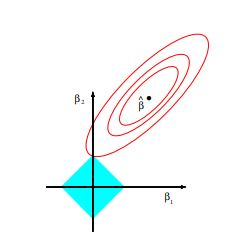
\includegraphics[width=0.5\textwidth]{Lasso_penalty}
	\caption{Lasso penalty and contour lines of least squares, NOTIZ: müssen wir selber erstellen das Bild}
	\label{lassopenalty}
\end{figure}

\subsubsection{Drawbacks}
%Problems with Lasso
\begin{enumerate}
	\item If two variables are highly correlated Lasso tends to pick only one of them and which one sometimes depends on minor changes. \todo{Man könnte im Appendix ein Minimalbeispiel wie wir es in Computational hatten zur Veranschaulichung geben.} If both variables are supposed to be selected, the estimation can be done via the elastic net. The elastic net was developed to overcome the problem of lasso not identifying highly correlated covariates. It minimizes the objective function $\| Y-X\beta\|_2^2+\lambda_1 \| \beta\|_1 +\lambda_2\|\beta\|_2^2$. The additional penalty has the advantage that it makes the objective function strictly convex.
	\item Lasso was designed for model selection and often has good predictive properties \citep{belloni2014}. However inference about model parameters such as regression coefficients has to be treated carefully. Lasso shrinks the coefficients of parameters and except for perfect model selecetion, can omit variables that have small influence in the model.
	\item Lasso does not exploit the structure of the regressors. If there is information on the regressor structure, e.g. the $X_i's$ can be ordered in a meaningful way or there are regressors that can be seen as a group, we would like to include this information in the estimation. Examples can be found in time series, biology, image reconstruction and many more.
	Lasso does not use the extra information when estimating. This gives rise to modifications of the Lasso, for example the fused lasso, which do so. 
\end{enumerate}


\subsection{Asymptotics}
\label{sec:asymptoticslasso}
-difficult - needs to use triangular arrays -urn example- assumptions diskutieren-min(n,p)=n
\bigskip

Asymptotics for high dimensional statistical interference is difficult. The reason is that for a meaningful analysis, besides $n$ also $p$ needs to go to infinity and it even has to grow faster than $n$. Else at some point, $n$ would be bigger than $p$ and so we wouldn't be in a high dimensional setting any more. As soon as $p << n$, we can preferably use known methods as OLS since they do not come with a shrinkage bias.  
The problem, when analyzing the asymptotics with growing $p$ is that the underlying statistical model/DGP is changing as $p$ grows. 
\bigskip

An easy example of this is that of an urn. Consider an urn with 10 red and 10 blue balls. We would like to estimate the probability of drawing a red ball by repeatedly drawing from the urn (with replacing). In high dimensional settings, each time we draw from the urn, the distribution of red and blue balls changes inside the urn. One way to handle high dimensional asymptotics is to work with triangular arrays.  For our linear model, this would be: $Y_{n;i}=\sum^{p_n}_{j=1}\beta^0_{n;j}X^{(j)}_{n;i}+\epsilon_{n;i}, \ i=1,...,n; \ n=1,2,...$. In the following, we will give results on prediction error accuracy, convergence of the estimator and variable screening. 
If we assume $||\beta^0||_1=||\beta_n^0||_1=o(\sqrt{\frac{n}{log(p)}}))$, $\epsilon$ as defined above and lambda in range of $\lambda=\lambda_n\asymp\sqrt{\frac{log(p)}{n}}$. The last assumption means that... . Then beta lasso is convergent in mean prediction sense. More formally $||X\hat{\beta}-X\beta^0||_2^2/n=o_P(1)$.
If the covariates are not too correlated and on the sparsity assumption then if lambda is in the range of $\lambda=\lambda_n\asymp\sqrt{\frac{log(p)}{n}}$ then beta converges in probability to $\beta$: $||\hat{\beta}(\lambda)-\beta^0||_1=o_P(1)$. 
We are interested if lasso is able to find the features with large coefficients. This is indeed the case as one can show that...


\subsection{Solution methods/algorithms}


%Lasso is a convec problem
The solutions to the minimization problem of the LASSO Estimator are the estimators $\hat\beta_\lambda$ that solve
$$\hat\beta_\lambda \in \argmin_{b\in \mathbb{R}^p}\underbrace{\frac{1}{n}\sum_{i=1}^{n}(y_i-x_i^Tb)^2+\lambda||b||_1}_{=S_\lambda (b)}.$$
%
Since the absolute value function is not differentiable at 0 we have to use subdifferential calculus, which is applicable because the objective is convex. In this simple case we can think of it as a widened interpretation of the derivative. The derivative of the absolute value function everywhere except at 0 is the sign function. So a quite natural idea is to say that the derivative of the function at 0 is characterized by the set $[-1,1]$. Calculating the left- and right-hand gradient leads to the Karush Kuhn tucker conditions for this problem.
\begin{align*}
b_\lambda \in \argmin_{\beta \in\rm \mathbb{R}^p} S_\lambda(b) \Leftrightarrow \begin{dcases} 
\frac{1}{n}\sum_{i=1}^n x_{ij}(y_i-x_i'b)= \frac{1}{2}\lambda sgn(\hat{\beta_{j}}) &\ if \quad \hat{\beta_j} \neq0 \\   
\frac{1}{n}\sum_{i=1}^n x_{ij}(y_i-x_i'b) \leq  \frac{1}{2}\lambda \ &\ if \quad \hat{\beta_j} =0
\end{dcases} 
\end{align*}
This often leads to numerous components $\hat\beta_{\lambda,j}$ of the estimators dropping to 0 as described in Theorem \eqref{theo: sparsity_lasso}. To illustrate this we first look at the reduced regression, i.e. the special case with $p=n$, where $X$ is the identity matrix and
$$Y_i=X \cdot\beta_i+\varepsilon_i=\sum^n_{j=1}1_{(j=i)}\beta_i+\varepsilon_i$$
%
Using the above conditions we see that the lasso estimator in this case is
$$\hat\beta_{\lambda,j}= \begin{dcases} y_j-\frac{n\lambda}{2} &if \quad y_j>\frac{n\lambda}{2}\\
            									  y_j+\frac{n\lambda}{2} &if \quad y_j<-\frac{n\lambda}{2}\\
                                                  0						 &if \quad |y_j|\leq \frac{n\lambda}{2}
\end{dcases}$$
This can be interpreted such that only $\hat\beta_{\lambda,j}$ that contribute more than $\frac{n\lambda}{2}$ to explaining $y$ are unequal to zero.\\ 
More formally, if we define $f_j(b)=\frac{1}{n}\sum^n_{i=1}(\varepsilon_i)x_{ij}=\frac{1}{n}\sum^n_{i=1}(y_i-x_i^Tb)x_{ij}$, then if $\beta_\lambda \in \arg\min_{b\in \mathbb{R}^p}$ this implies that for all $b_{\lambda,j}=0$, $|f_j(b_\lambda)|\leq \frac{1}{2}\lambda$. \\
Since the optimization problem consists of sums of convex functions, computing the lasso estimator is in itself a convex optimization problem. That means we can use powerful algorithms to find the solution path. \todo{An dieser Stelle sollten wir kurz und knapp den LARS Algorithmus erwähnen.} \newline


%algorith for estiumation lasso
%
%
% lambda
\subsubsection{Coordinate descent} \label{Sec: Coordinate Lasso}
For fixed $\lambda_1$ the lasso estimator can be calculated by the coordinate descent algorithm. We can use coordinate descent because the objective function has the structure which is necessary for the algorithm to converge to the global minimum. The structure is
\begin{equation}
g(\beta_1,...,\beta_p)+\sum_{j=1}^Ph_j(\beta_j) \nonumber
\end{equation}
where $g: \mathbb{R}^p \to \mathbb{R}$, differentiable and convex and $h_j(\beta_j)$ are convex. The squared Euclidean norm and the absolute value functions fulfill these criteria. An important observation is that the functions only depend on one $\beta$ coefficient.
\cite[chapter 5]{sparsity}
\todo{Näher erklären warum Lasso es erfüllt und was cross-validation überhaupt ist}

\section{Fused Lasso}
\subsection{Definition and set-up}

Consider the same $Y=X\beta+\varepsilon$ setting as for the lasso, but with one extension. Assume that there is a structure in $\beta$, such that neighboring $\beta_i$'s often have equal values.\\
In that case, Lasso does not exploit the structural information within the features. However this structure can be exploited by adding a second penalty term that penalizes differences between neighboring $\beta_i$'s, i.e. $\lambda_2\sum_{j=2}^p|\beta_j- \beta_{j-1}|$. Adding this penalty term to Lasso's objective function, leads to the fused lasso estimator 
	\begin{equation}
		\hat{\beta}_{\lambda_1,\lambda_2}^{FL}=\argmin_{\beta \in\rm \mathbb{R}^p} \left\{ \frac{1}{2n}  \sum_{i=1}^{N}(y_{i}-x_{i}'\beta)^2+\lambda_1 \sum_{j=1}^p|\beta_j|+ \lambda_2 \sum_{j=2}^p|\beta_j- \beta_{j-1}| \right \}.
	\end{equation}
	
	
\subsection{Properties}

\subsubsection{The penalty constants}
In contrast to the lasso case, we have two penalty constants. $lambda_1$ is the coefficient on the lasso penalty and influences the estimator in the same way. $\lambda_2$ is the coefficient on the fusion penalty. For $\lambda_2=0$, we remain in the lasso problem. For an increasing $\lambda_2$, more and more neighboring $\beta_j$'s get 'fused' together, in the sense that $\beta_j=\beta_{j-1}$. For $\lambda_2\to\infty$, the objective function is only minimized if $\sum_{j=2}^p|\beta_j- \beta_{j-1}|$.\\
As for the lasso, the penalty constants have to be chosen by the researcher. A possible approach could be crossvalidation on a two dimensional grid, as proposed by \citep{fused}. In that case an upperbound for $\lambda_1$ should be the optimal $\lambda$ of the lasso estimator.

\subsubsection{Properties of the solution}

Similar to the Lasso, we can define the following properties of the Fused Lasso estimator.
\todo{speak about prior information that is incorporated.}

\begin{theorem}
	\begin{enumerate}
		\item[]
		\item \textbf{Existence} A solution of the minimization problem always exists.
		\item \textbf{Piecewise Constant}
		
\citet{rosset2007piecewise} give conditions under which the solution path of a regularized optimization problem is linear. They give conditions for a slightly different penalty term class but in chapter 5.2 they argue that the fused lasso is also piecewise constant.
	\end{enumerate}
\end{theorem}
\todo{Brauchen eine Interpretation der piecewise constant eigenschaft, averaging of the coefficients, außerdem müssen wir beschreiben wieso diese Eigenschaft wertvoll ist.}
\todo{In der Mathematik heißt eine Funktion $f\colon T\to M$ von einem topologischen Raum $T$ in eine Menge $M$ lokal konstant, wenn für jedes $x\in T$ eine Umgebung $U$ von $x$ existiert, auf der $f$ konstant ist.}


\begin{theorem}[Sparsity of Fused Lasso] \citep{fused}
	Let $n_{seq}(\beta) = \sum_{j=1}^{p} \mathbbm{1} \{\beta_j \neq \beta_{j-1}\}$, i.e. the number of sequences of identical non-zero coefficients. Then under 'non-redundancy' conditions on the design matrix $X$, the fused lasso estimator is unique and we have $\hat{\beta}$ with $n_{seq}(\hat{\beta}) \leq N$.
\end{theorem}


\subsection{Asymptotics}

In the following we cite an asymptotic result from \citet{fused} and give an interpretation hereof.
For simplicity the authors assumed that $p$ is fixed with $N \rightarrow \infty$. As the authors note themselves these are ``not particularly realistic asymptotic conditions'' as the lasso and fused lasso are methods for high-dimensional data, which is not the case any more if $N$ gets larger than $p$. The methods to deal with such a scenario are difficult (as described in section \ref{sec:asymptoticslasso}). Still we think that the interpretation of the result is insightful.

\begin{theorem}
	If $\lambda_N^{(l)}/\sqrt{N} \rightarrow \lambda_0^{(l)} \geq 0 \  (l=1,2)$ and
	\begin{equation*}
		C = \lim\limits_{N \rightarrow \infty}{(\frac{1}{N} \sum_{i=1}^{N}x_i x_i^T)}
	\end{equation*}
	is non-singular then
	\begin{equation*}
		\sqrt{N}(\hat{\beta}_N - \beta) \rightarrow_{\text{d}} \argmin(V),
	\end{equation*}
	where
	\begin{align*}
		V(u) = &-2u^T W + u^T Cu + \lambda_0^{(1)} \sum_{j=1}^{p} \{u_j \sgn(\beta_j)I(\beta_j \neq 0) + |u_j|\ I(\beta_j=0) \} \\
		&+ \lambda_0^{(2)} \sum_{j=2}^{p} \{(u_j - u_{j-1}) \sgn(\beta_j - \beta_{j-1})I(\beta_j \neq \beta_{j-1}) + |u_j-u_{j-1}|\ I(\beta_j=\beta_{j-1}) \} 
	\end{align*}
and $W$ has an $\mathcal{N}(0,\sigma^2 C)$ distribution.
\end{theorem}

The idea of the theorem and proof is similar to that in \citep{asymptoticslasso} where the asymptotics of the Lasso are analyzed. In order to study the limiting behavior of the fused lasso the asymptotic behavior of a specific objective function is studied. This objective function is minimized at $\sqrt{N}(\hat{\beta}_n-\beta)$ and converges in distribution to $V(u)$. The proof of the theorem can be found in \citep{fused}, we will give an interpretation of the result.
\smallskip

\noindent As $n$ grows to infinity, we need to modify the penalty constant too. That means we need to let $\lambda$ grow as well in a particular speed, this means concretely that $\lambda_N^{(l)}/\sqrt{N} \rightarrow \lambda_0^{(l)} \geq 0 \  (l=1,2)$, so $\lambda$ is $o(n)$ \todo{Describe this further.}
\smallskip

\noindent First we take a closer look at the function $V(u)$. Only the first part of the function is stochastic. The second part can be seen as a bias term as we will describe no further.
\smallskip

\noindent Let us start with the case, where $\lambda_0^{(1)}= \lambda_0^{(2)} = 0$, so we are back to OLS. The function $V(u)$ reduces to $V(u) = -2u'W + u'Cu$. It is easy to see that this is minimized at $C^{-1}W$, so as expected 		$\sqrt{N}(\hat{\beta}_N - \beta) \rightarrow_{\text{d}} \mathcal{N}(0,\sigma^2 C^{\frac{1}{2}})$.
When $\lambda_0^{(1)}$ and/or $\lambda_0^{(2)}$ are unequal to zero we will not get asymptotic normality centered at zero.

%Tibshirani et al. define $V_N(u)$ by
%\begin{align*}
%	V_N(u)= &\sum_{i=1}^{N} \{(\varepsilon_i - u^Tx_i/\sqrt{N})^2 -\varepsilon_i^2 \} + \lambda_N^{(1)} \sum_{j=1}^{p}(|\beta_j + u_j / \sqrt{N}|-|\beta_j|) \\
%	&+ \lambda_N^{(2)} \sum_{j=2}^{p} \{ |\beta_j - \beta_{j-1}+(u_j-u_{j-1})/\sqrt{N}|-|\beta_j - \beta_{j-1}|\}.
%\end{align*}
%
%The design of $V_N(u)$ is such that it is minimized at $\sqrt{N}(\hat{\beta_n}-\beta) $. \todo{Could prove this}
%Furthermore they show that $V_N(u) \rightarrow_{\text{d}} V(u)$ with finite-dimensional convergence holding as well \citep{fused}.
%They conclude that since $V_N$ is convex and $V$ has a unique minimum, it follows that \todo{Need an explanation of this fact since the reference paper is not online}
%\begin{equation*}
%	\argmin(V_N) = \sqrt{N}(\hat{\beta_N}-\beta) \rightarrow_{\text{d}} \argmin(V).
%\end{equation*}


Interpretation of the result: Nonzero parameters are estimated with some asymptotic bias if $\lambda_0 > 0$. When some of the $\beta_j$s are exactly $0$, the limiting distributions put positive probability at $0$. 

\subsection{Solution methods/algorithms}

\subsubsection{Coordinate Descent}
In section \ref{Sec: Coordinate Lasso} we saw that the conditions for the coordinate descent to be a suitable solution method are fulfilled for the lasso. Unfortunately for the fused lasso this is not the case. The reason is that the separated non differentiable functions $h$ do not only depend on a single coefficient but on two. Take for example the fused signal approximator case, where we can set $\lambda_1 = 0$ (compare lemma \ref{sa: soft thresholding}). 
%Assume we have $p=100$ and coordinate descent sets the coefficients successfully to their optimal value. 
Assume that the previous iteration step set $\hat{\beta}_1=\hat{\beta}_2$ and we are in the new iteration step, where we minimize over $\beta_1$. Observe any change in $\beta_1$ introduces an increase of the absolute value of the difference of $\hat{\beta}_1$ and $\hat{\beta}_2$. Let us consider a situation in which it would be optimal to increase $\hat{\beta}_1$ a little to get rid of some squared differences in the model fit, but the difference in the absolute value is larger, so it is optimal for $\hat{\beta}_1$ to stay as in the previous iteration step. Assume we face the same problem in the iteration step for $\beta_2$, i.e. increasing it a little would be better for model fit, but it isn't done because of the combined penalty.
in such a scenario coordinate descent gets stuck. Therefore we have to use algorithms like gradient descent because they can move $\beta_1$ and $\beta_2$ simultaneously, so that here both increase slightly, so that the squared error gets smaller and the absolute difference stays 0.
A path algorithm is explained in the next section.
\cite[chapter 5]{sparsity}

%For the calculation of the solution one can make use of the following handy property of the fused lasso.
%
%
%\begin{lemma} \label{sa: behavior of optimum}[Behavior of the optimum] (cf. \citep{sparsity})
%	For any $\lambda_1' > \lambda_1$, we have
%	\begin{equation}
%		\hat{\beta_i}(\lambda_1', \lambda_2) = S_{\lambda_1'-\lambda_1} (\hat{\beta_i}(\lambda_1, \lambda_2)) \text{ for each } i = 1, \ldots, N,
%	\end{equation}
%	where $S$ is the soft-thresholding operator $S_\lambda(z) := \sgn(z)(|z|-\lambda)_+.$
%\end{lemma}
%\noindent	One important special case of Lemma \ref{sa: behavior of optimum} is the following equality, on which the path algorithm for the solution, which will be described in the next section, is based.

%\begin{equation}
%	\hat{\beta_i}(\lambda_1, \lambda_2) = S_{\lambda_1} (\hat{\beta_i}(0, \lambda_2)) \text{ for each } i = 1, \ldots, N.
%\end{equation}

\subsection{Fused Lasso Signal Approximator}

A special case of the fused lasso occurs when the predictor matrix is the $N \times N$ identity matrix. In this case the estimator has the following form.

	\begin{equation}
	\hat{\beta}_{\lambda_1,\lambda_2}^{FLSA}=\argmin_{\beta \in\rm \mathbb{R}^p} \left\{ \frac{1}{2n}  \sum_{i=1}^{N}(y_{i}-\beta_i)^2+\lambda_1 \sum_{j=1}^p|\beta_j|+ \lambda_2 \sum_{j=2}^p|\beta_j- \beta_{j-1}| \right \}	
 \label{Fused-Signal}	\end{equation}

We can interpret the estimator as an approximator of an unknown signal which is blocky and sparse in its nature and corrupted by an additive noise. (cf. \citep{rinaldoproperties})

\begin{lemma}[Soft thresholding property] \label{sa: soft thresholding} (cf. \cite{sparsity})
	For any $\lambda_1' > \lambda_1$, we have
		\begin{equation}
		\hat{\beta_i}(\lambda_1', \lambda_2) = S_{\lambda_1'-\lambda_1} (\hat{\beta_i}(\lambda_1, \lambda_2)) \text{ for each } i = 1, \ldots, N,
		\end{equation}
	where $S$ is the soft-thresholding operator $S_\lambda(z) := \sgn(z)(|z|-\lambda)_+.$
\end{lemma}
	\noindent	One important special case of Lemma \ref{sa: soft thresholding} is the following equality, on which a lot of path algorithms for the solution are based.
	
	\begin{equation}
		\hat{\beta_i}(\lambda_1, \lambda_2) = S_{\lambda_1} (\hat{\beta_i}(0, \lambda_2)) \text{ for each } i = 1, \ldots, N.\footnote{Proofs of lemma \ref{monotone_fusion} and lemma \ref{sa: soft thresholding} can be found in the appendix.}
	\end{equation}
	
Another useful property of the fused lasso estimator (only) in this easy setting is that of monotone fusion.

\begin{lemma}[Monotone Fusion] (cf. \citep{sparsity}) \label{monotone_fusion}
	Suppose that for some value of $\lambda$ and some index $i \in \{1, ..., -1 \}$ the optimal solution satisfies $\hat{\beta_i}(\lambda)$ = $\hat{\beta}_{i+1}(\lambda)$. Then for all $\lambda' > \lambda$, we also have $\hat{\beta_i}(\lambda')$ = $\hat{\beta}_{i+1}(\lambda')$.
\end{lemma}

\newpage
\section{Simulation}

In this section we want to illustrate the theory that was elaborated on above.
One of the main goals of our estimators is model selection. That means in order to analyze how well the estimators perform on our simulated data we need to analyze their so called specificity and sensitivity. Specificity means the proportion of the true zero coefficients and sensitivity the proportion of the true non-zero coefficients that are detected by the estimated model.



\newpage

\todo{think about different structures of the beta-vector (which supports using one of the estimators)}
Possible structures of coefficients for the simulation:
\begin{enumerate}
	\item plateaus (of different size) already implemented
	\item plateaus and one(ore more) peaks
	\item sparsity, but without plateaus
	\item situations in which the lasso or fused lasso may not be appropriate (imposing a wrong prior):
	\begin{enumerate}
		\item no ordering of the features
		\item no sparsity
	\end{enumerate}
\end{enumerate}

\todo{Insert images from simulation and evaluation. Müssen package booktabs benutzen.}


\section{Real Data Application}

\subsection{Comparative Genomic Hybridization Data}
The first application we want to consider is from medical science. We want to look at data from Comparative Genomic Hybridization (CGH), a powerful method for molecular analysis of cancer.    
CGH provides an overview of changes in DNA sequence copy number in a tumor sample 
%and maps these changes on normal chrosomosomes
relative to a control sample, i.e. normal chromosomes. Changes can be in form of losses, deletions, gains and amplifications\citep{cghmain}. The DNA  sequence copy number is then given as a function of chromosomal location throughout the entire genome, the genetic material of an organism \citep{cghsecond}. This can for example look as in figure (\ref{cghdata}).
hi
\begin{figure}
	\centering
	\includegraphics[width=\textwidth]{../../out/figures/red_line.pdf}
	\caption{CGH Data}
	\label{cghdata}
\end{figure}

The CGH data are coming from an experiment and are very noisy. This renders some kind of smoothing necessary before analysing the data. \\
Biological considerations dictate that it is typically segments of a chromosome — rather than individual genes — that are replicated, Consequently, we might expect that the underlying vector of true copy numbers to be piecewise-constant over contiguous regions of a chromosome.
In this specific example we have as many regressors (genes) as observations (copy numbers) \citep{sparsity}.
As seen above the fused lasso signal approximator is designed for cases like these with $ p = n$ and a meaningful ordering of the coefficients.

\subsection{Other application}
\todo{look for other application with $p>n$, e.g. Spectral Data or datasets from Elements of Statistical Learning} 

\section{Conclusion/Discussion}

\begin{enumerate}
	\item Neighbors generalize to neighboring areas  (for example image reconstruction for 2d case, cf. \citep{sparsity})
	\item Several different choices for the penalties on neighboring coefficients (apart from the $\ell^1$-norm) are possible.
	\item Assume a uniformly spaced index, can consider cases where the index variable has nonuniform values (see p.667 in \citep{sparsity})
	\item Can consider case where the features are unordered.
\end{enumerate}
 %\citep{adams1995hitchhiker}
 
 \citep{elements}

\appendix

\newpage

\section{Code}


\lstset{language=Python}
\lstset{frame=lines}
\lstset{caption={Fused Lasso Signal Approximator}}
\lstset{label={lst:code_direct}}
\lstset{basicstyle=\footnotesize}
\begin{lstlisting}
import numpy as np
import pandas as pd
import random as rd
import matplotlib.pyplot as plt
from scipy.interpolate import UnivariateSpline
from scipy.optimize import minimize
import time


start_time = time.time()
np.random.seed(1)
rd.seed(5)


y = np.random.normal(0, 5, 30)

y[5:8] = y[5:8]-y[5:8] + 10 + np.random.normal(0,1,3)


#y[15:18] = y[15:18]-y[15:18] - 20 + np.random.normal(0,1,3)

data = np.loadtxt("cgh.txt", delimiter=',')

#y = [1,2,3,4,5,6,7,8,9,10,10.001]

#y = [1,-3,5,-7,9,-11,11.001]

def group_minimize_np(a,b,y,lambda2,p):
    
    container12 = np.ones((len(b),2))
    
    container12[:,0] = a
    container12[:,1] = b
    
   # beta123 = np.ones(p)
    
    number_of_groups2 = len(container12)
    
    
    beta123 = np.repeat(a,b.astype(int))
    
   
            
            
    return 0.5*(np.sum((y-beta123)**2))+lambda2 * 
    np.sum(
    np.abs(
    container12[:,0][0:number_of_groups2-1]-container12[:,0][1:number_of_groups2]
    ))
        



def fused_signal_approximation(y):
   
    
  
    # Initialization
    p = len(y)
    beta = np.array(y)
    
    container = np.ones((p,2))
    container[:,0] = y
    container[:,1] = np.ones(p)
    
    beta_matrix = np.ones((p,1))
    beta_matrix[:,0] = y
    
    
    lambda_vector = np.array([])
    
    lambda2 = 0
    lambda_vector = np.append(lambda_vector,[lambda2])
    
    
    
    while lambda2 < 5000:#for i in list(range(40)):#len(container[:,0]) > 1:
    
        
        group_count = len(container[:,1])
        
        ##Calculating hitting time
        
        # Calculating differences
        difference = beta[0:group_count-1] - beta[1:group_count]
        
        
        #calculate derivatives
        beta_deriv_container = np.ones(group_count)
        
        for j in list(range(group_count)):
            
            
            
            if j == 0:
                beta_deriv_container[j] = (-1/container[j,1]) * 
                (np.sign(container[j,0]-np.sign(container[j+1,0])))
            elif j == len(container[:,1])-1:
                beta_deriv_container[j] = (-1/container[j,1]) * 
                (np.sign(container[j,0]-np.sign(container[j-1,0])))
            else:
                beta_deriv_container[j] = (-1/container[j,1])* 
                (np.sign(container[j,0]-np.sign(container[j-1,0])+ 
                np.sign(container[j,0]-np.sign(container[j+1,0]))))
         
            
        ## Calculating differences in derivatives    (Nenner)
        difference_clean_deriv = beta_deriv_container[1:group_count] - 
        beta_deriv_container[0:group_count-1]
        
        ##calculating hitting time
        h = np.divide(difference,difference_clean_deriv) + lambda2
        
        
        min nur ueber Werte groesser als das alte lambda sind
        
        h[h < lambda2] = 10000
        
        lambda2 = np.amin(h)
        
        
        
        #sammeln der lambdas in jeder iteration
        lambda_vector = np.append(lambda_vector,[lambda2])
        
        
        
        ## hitting time indices
        fuse_set_1 = np.argmin(h)
        fuse_set_2 = np.argmin(h) + 1
        
        
        ## update container group column
        container[fuse_set_1,1] = container[fuse_set_1,1]   + container[fuse_set_2,1]
        
        container = np.delete(container, (fuse_set_2), axis=0)
        #print(container)
        
        # startwert fuer den optimierer
        
        #x0 = np.ones(len(container[:,1]))
        x0 = container[:,0]
        
        ##update beta
        beta_opt = minimize(
        group_minimize_np, x0,args=(container[:,1],y,lambda2,p), method='Nelder-Mead', 
        options={'xtol': 1e-8, 'disp': True, 'maxiter' : 1000000}) 
        
        
       
        ## add new beta to container
        container[:,0] = beta_opt['x']
        
        
        ### For given updated container fill beta_matrix
        
        aux = np.array([np.repeat(container[:,0],container[:,1].astype(int))]).T
        
        beta_matrix = np.concatenate((beta_matrix,aux),axis =1)
        
        

    
    # PLot 
    beta_matrix = pd.DataFrame(beta_matrix)
    lambda_vector = pd.DataFrame(lambda_vector)
    y = pd.DataFrame(y)
    for i in list(range(len(lambda_vector))):
        
        
        
        d = beta_matrix.iloc[i,0:len(lambda_vector)-1]
        c = lambda_vector.iloc[0:-1]
        s = UnivariateSpline(c, d,k=1)
        
        plt.plot(c, d, '.-')
        
    return plt.plot(c, d, '.-'), beta_matrix,lambda_vector, container
        
      
Plot, beta_Matrix,lambda_vector, container = fused_signal_approximation(data[0:100])

#fused_signal_approximation(data[0:100])


print(Plot)      
 
print(lambda_vector)

print(pd.DataFrame(beta_Matrix))

print(container)   
                                                            
print("My program took", time.time() - start_time, "to run"  )  


plt.plot(data[0:100])
plt.plot(beta_Matrix.iloc[:,40])
\end{lstlisting}
\lstset{caption={Solution Path Lasso}}

\begin{lstlisting}
import numpy as np
import matplotlib.pyplot as plt
from scipy.interpolate import UnivariateSpline
import pandas as pd
import random as rd


def easy_lasso(y,l):
    y = np.array(y)
    n = len(y)
    
    y[y>n*l/2] = y[y>n*l/2] - n*l/2
    y[y<-n*l/2] = y[y<-n*l/2] + n*l/2
    y[np.abs(y) <= n*l/2] = 0
    
    b = y
    
    return b

y = np.random.normal(0, 100, 10)
#data = np.loadtxt("cgh.txt", delimiter=',')

def solution_path(y):
    
    n = len(y)
    
    lambda_container = np.array([])
    
    lambda1 = 0
    lambda_container = np.append(lambda_container,[lambda1])
    
    beta_matrix = np.ones((n,1))
    beta_matrix[:,0] = y
    
    
    
    while sum(y) != 0:
        
        lambda_container_loop = np.ones(n)
        
        for i in list(range(n)):
            
            if y[i] > n*lambda1/2:
                
                lambda_container_loop[i] = y[i]*2/n
                
                
                
            elif y[i] <-n* lambda1 /2:
                
                lambda_container_loop[i] = -y[i]*2/n
                
                
            else:
                lambda_container_loop[i] = 10000
                
                
        lambda_container_loop[lambda_container_loop < lambda1] = 10000
        lambda1 = np.amin(lambda_container_loop)
        lambda_container = np.append(lambda_container,[lambda1])
        
        y = np.array(easy_lasso(y,lambda1))
        y = np.reshape(y, (-1, n)).T
        beta_matrix = np.concatenate((beta_matrix,y),axis = 1)
        
        
        beta_matrix123 = pd.DataFrame(beta_matrix)
        lambda_container = pd.DataFrame(lambda_container)
        for i in list(range(len(lambda_container))):
            
            
            
            d = beta_matrix123.iloc[i,0:len(lambda_container)]
            c = lambda_container
            #s = UnivariateSpline(c, d,k=1)
            
            plt.plot(c, d, '.-')
        
        
        
        
    return beta_matrix, lambda_container
    
Beta_Matrix, Lambda_Container = solution_path(y)

#for i in list(range(63)):

    #plt.plot(Beta_Matrix[:,i])


    
    

\end{lstlisting}

\todo{Insert code for simulation with lasso and fused lasso as soon as the question is being answered how to optimize over both lambdas}


\section{Proofs}

Equivalence of (\ref{Primal}) and (\ref{LassoLambda}):
First of all note that for any $b$ with $||b||_1 > \frac{||Y||^2}{\lambda}$ the following inequality holds:
\begin{equation}
	S_\lambda(b) \geq \lambda ||b||_1 > ||Y||^2 = S_\lambda(0).
\end{equation}

that means the Lasso criterion is smaller for $\tilde{b}=0$, so $b$ is not a solution.
Thus we have
\begin{equation*}
 \hat{\beta}_\lambda^{Lasso} = \argmin_{\beta \in\rm \mathbb{R}^p} S_\lambda(b) = \argmin_{\substack{\beta \in\rm \mathbb{R}^p\\ ||b||_1 \leq \frac{||Y||^2}{\lambda}}} S_\lambda(b)
\end{equation*}
so the two ways of writing the estimator are equivalent.

\begin{proof} Convexity of solution set \newline
\todo{Diese Aussage lässt sich verallgemeinern, sodass $\beta_1$ und $\beta_2$ Schätzer mit verschiedenen Lambdas sein können, würde ich auch machen, da es ein sehr spezieller Fall ist, dass es zwei Lösungen für das gleiche Lambda gibt}
Define the objective function
\begin{align*}
h(\beta)=\|Y-X\beta\|_2^2+\lambda\|\beta\|
\end{align*}
Note that $h(\beta)$ is convex. Let $\beta_1$ and $\beta_2$ be two minimizers of $h(\beta)$ and let $\beta_3=\alpha\beta_1+(1-\alpha)\beta_2$ where $\alpha \in (0,1)$. Then due to convexity of $h(\beta)$ for any $\beta \in \mathbb{R}^p$ we have
\begin{align*}
h(\beta_3)&=h(\alpha\beta_1+(1-\alpha)\beta_2) \leq \alpha \underbrace{h(\beta_1)}_{\leq h(\beta)}+(1-\alpha)\underbrace{h(\beta_2)}_{\leq h(\beta)} \\ &\leq \alpha h(\beta)+(1-\alpha)h(\beta)=h(\beta) \\ &\Rightarrow \alpha\beta_1+(1-\alpha)\beta_2 \ \ \ \text{is also a minimizer}
\end{align*}
Note that this implies that in case of two solutions there are uncountably many solutions.
\end{proof}

\begin{proof} Existence \newline
Consider the problem written as in (\ref{Primal}). Observe that the arg min is taken over a compact set and the squared $\ell^2$ norm is a continuous function. By the extreme value theorem it follows that there always exists at least one solution to the minimization problem.
\end{proof}

\todo{Ich finde die Notation in dem Beweis nicht gelungen, für Fused Lasso hatten wir die Lambdas bisher unten und nicht oben, einige Typos müssen korrigiert werden.}
\begin{proof} Lemma \ref{sa: soft thresholding} (The basis of this proof can be found in \citep{friedman2007pathwise})
	We want  to show that the solution to this problem 
	\begin{equation}
	\frac{1}{2}  \sum_{i=1}^{6}(y_{i}-\beta_i)^2+\lambda_1\sum_{i=1}^p|\beta_i| + \lambda_2 \sum_{j=2}^6|\beta_j- \beta_{j-1} |
	\end{equation} is equivalent to first calculate the solution for some lambda2  and $\lambda_1 =0$ and then soft thresholding it with $\lambda_1>0$. We argue as follows: the soft thresholded estimator also solves the gradient equation which is necessary and sufficient for it to be a solution. The gradient function for some $\beta_j$ is given by
	\begin{equation}
	-(y_j-\hat{\beta}_j)+\lambda_1 sgn(\beta_j)+\lambda_2 [sgn(\hat{\beta}_j-\hat{\beta}_{j-1})+sgn(\hat{\beta}_{j+1}-\hat{\beta_j})]=0
	\end{equation}
	Assume we calculated a solution for $\lambda_1=0$ and $\lambda_2 > 0$ denoted by $\hat{\beta^0}$. The soft thresholded version of it is given by $\hat{\beta^{\lambda_1}}=sgn(\hat{\beta^0})(|\hat{\beta^0}|-\lambda_1)^{\text{+}}$. The next step is that we plug it into the above equation and argue that it holds. Before we note some observations. Note that if $\hat{\beta}^0_j=0$ then we are free to choose $sgn(\hat{\beta}^0_j) \in [-1,1]$, for convenience we set it to 0. Next we compare the differences $sgn(\hat{\beta}_j^0-\hat{\beta}_{j-1}^0)$ with $sgn(\hat{\beta}_j^{\lambda_1}-\hat{\beta}_{j-1}^{\lambda_1})$. There are two cases: if after the thresholding one parameter is set to 0 and the other one unequal to zero we know that betas just changes in the level so the differences stays the same, the other case is if both get shrunken to zero, then since $sgn(0)$ we are free to choose the value, especially we can set equal to the non thresholded estimators. So it follows $sgn(\hat{\beta}_j^0-\hat{\beta}_{j-1}^0)=sgn(\hat{\beta}_j^{\lambda_1}-\hat{\beta}_{j-1}^{\lambda_1})$. Finally we can plug the soft thresholded estimator in the derivative condition.
	\begin{align}
	-y_j+sgn(\hat{\beta}^0_j)(|\hat{\beta}_j^0|-\lambda_1)^{\text{+}}+\lambda_1 sgn(\hat{\beta}_j^{\lambda_1})+\lambda_2 [sgn(\hat{\beta}^{\lambda_1}_j-\hat{\beta}^{\lambda_1}_{j-1})+sgn(\hat{\beta}^{\lambda_1}_{j+1}-\hat{\beta}^{\lambda_1}_j)]=0
	\end{align}
	Consider the case  where $|\hat{\beta^0}|-\lambda_1\geq0$, noting the equality $sgn(\beta)|\beta|=\beta$ and the fact that the sign of the differences is the same as for lambda equal to we are left with
	\begin{equation}
	-y_j+\hat{\beta}_j^0-\lambda_1 sgn(\hat{\beta}^0_j) + \lambda_1sgn(\hat{\beta}^{\lambda_1}_j)+\lambda_2 [sgn(\hat{\beta}^{0}_j-\hat{\beta}^{0}_{j-1})+sgn(\hat{\beta}^{0}_{j+1}-\hat{\beta}^{0}_j)]=0
	\end{equation}
	So by setting $sgn(\hat{\beta}^0_j)=sgn(\hat{\beta}^{\lambda_1}_j)$ equation 20 reduces to the optimality condition if lambda1 is equal to 0 and since we assumed $\hat{\beta}^0$ is the solution for this problem we know the equation holds.
	In case two if $|\hat{\beta}_j^0|-\lambda_1<0$ then $\hat{\beta}_j^{\lambda_1}=sgn(\hat{\beta}_j^0)(|\hat{\beta}_j^0|-\lambda_1)^{\text{+}}=0$. Ignoring by the same arguments the sign differences we are left with
	\begin{equation}
	-y_j+\lambda_1 sgn(\hat{\beta}_j^{\lambda_1})
	\end{equation}
	Since we can chose the sign to be anywhere between -1 and 1 we set it to $\frac{\hat{\beta}_j^{0}}{\lambda_1}$
\end{proof}

\begin{proof} Idea: Monotone Fusion Property \citep{friedman2007pathwise}
For simplicity we assume soft thresholding property is true. That means we can set $\lambda_1=0$ and we have n=p=6. Then the objective function looks as follows
\begin{equation}
\frac{1}{2}  \sum_{i=1}^{6}(y_{i}-\beta_i)^2+ \lambda_2 \sum_{j=2}^6|\beta_j- \beta_{j-1} |
\end{equation}
Let's assume we know the solution and it satisfies $\hat{\beta}_3=\hat{\beta}_4=\hat{\beta}_5=\hat{\beta}^*$ and $\hat{\beta}_2\neq\hat{\beta}^*$ and $\hat{\beta}_6\neq\hat{\beta}^*$ It follows that $sgn(\hat{\beta}_3-\hat{\beta}_2)$ and $sgn(\hat{\beta}_6-\hat{\beta}_5)$ are both $\in \{-1,1\}$ further $sgn(\hat{\beta}_4-\hat{\beta}_3)$ and $sgn(\hat{\beta}_5-\hat{\beta}_4)$ vary in $[-1,1]$. The partial derivative's of the objective function evaluated at the solution are given by
\begin{align}
-(y_1-\hat{\beta}_1)+\lambda_2 sgn(\hat{\beta}_2-\hat{\beta_1})=0 \\
-(y_2-\hat{\beta}_2)+\lambda_2 [sgn(\hat{\beta}_2-\hat{\beta_1})+sgn(\hat{\beta}_3-\hat{\beta_2}))]=0 \\
-(y_3-\hat{\beta}_3)+\lambda_2 [\underbrace{sgn(\hat{\beta}_3-\hat{\beta_2}}_{Boundary})+sgn(\hat{\beta}_4-\hat{\beta_3})]=0 \\
-(y_4-\hat{\beta}_4)+\lambda_2 [sgn(\hat{\beta}_4-\hat{\beta_3})+sgn(\hat{\beta}_5-\hat{\beta_4})]=0 \\
-(y_5-\hat{\beta}_5)+\lambda_2 [sgn(\hat{\beta}_5-\hat{\beta_4})+\underbrace{sgn(\hat{\beta}_6-\hat{\beta_5})}_{Boundary}]=0 \\
-(y_6-\hat{\beta}_6)+\lambda_2 [sgn(\hat{\beta}_6-\hat{\beta_5})+sgn(\hat{\beta}_7-\hat{\beta_6})]=0 
\end{align}
Since the sgn functions which evaluate exactly to -1 or 1 are fixed ,they can be seen as boundaries for the "inner" differences. And so the inner differences only depend on  a sub system of the above equations. The differences $(12)-(11)$ and $(11)-(10)$ can be written as. 
\begin{align}
\left(\begin{matrix}2&-1\\-1&2\end{matrix}\right)\left(\begin{matrix}sgn(\hat{\beta}_4-\hat{\beta_3})\\sgn(\hat{\beta}_5-\hat{\beta_4})\end{matrix}\right)&=\frac{1}{\lambda_2} \left(\begin{matrix}y_4-y_3\\y_5-y_4\end{matrix}\right) + \left(\begin{matrix}sgn(\hat{\beta}_3-\hat{\beta_2})\\sgn(\hat{\beta}_6-\hat{\beta_5})\end{matrix}\right) \\ \Rightarrow \left(\begin{matrix}sgn(\hat{\beta}_4-\hat{\beta_3})\\sgn(\hat{\beta}_5-\hat{\beta_4})\end{matrix}\right)&=\frac{1}{\lambda_2} \left(\begin{matrix}\frac{1}{2}&\frac{1}{4}\\\frac{1}{4}&\frac{1}{2}\end{matrix}\right)   \left(\begin{matrix}y_4-y_3\\y_5-y_4\end{matrix}\right) \\ &+  \left(\begin{matrix}\frac{1}{2}&\frac{1}{4}\\\frac{1}{4}&\frac{1}{2}\end{matrix}\right)      
  \left(\begin{matrix}sgn(\hat{\beta}_3-\hat{\beta_2})\\sgn(\hat{\beta}_6-\hat{\beta_5})\end{matrix}\right)
\end{align}
Note that both entries in (16) are always between -1 and 1. We also know that the sgn function in (15) are between -1 and 1. If $\lambda:2$ increases it only shrinks the values closer to 0. Thus we see $\hat{\beta}^*$ might change but that fused set remains constant. Since the structure of the solution remains intact. Only if a new beta joins the group say beta2, but then we could repeat the same argument.
\end{proof}


\listoftodos


\newpage
\bibliography{refs}

\end{document}

%
%\section{Lasso}
%    \subsection{Characterization of the LASSO-Solution}
%    For the Lasso criterion  
%    $$ \min_{b\in\RR^p}S_\lambda(b)=\frac{1}{n}(y_i-X_i^Tb)^2+\lambda||b||_1,\qquad \lambda>0$$
%    there exists $ b_\lambda\in\argmin_{b\in R^p}S_\lambda(b)$.\footnote{Proof: For }

